\section{Experimental Results and Discussion}

\subsection{Experimental Setup}

\subsubsection{Dataset}

The framework was evaluated on 43 real-world CCTV video sequences from the Snatch 1.0 benchmark and supplementary surveillance footage, comprising 96,926 frames across 3,877.05~s (64.62~min). The dataset contains 35 positive chain-snatching sequences and 8 negative control sequences of normal surveillance. The recordings encompass heterogeneous surveillance conditions, including varied spatial resolutions, frame rates, static outdoor camera views, daytime, mixed-lighting, and night-time lighting environments.

\subsubsection{Ground Truth and Evaluation Protocol}

Binary video-level ground-truth annotations were provided for all 43 sequences (35 positive, 8 negative), with temporal interaction boundaries established for snatching events. Annotations also cover standard action categories (Walking, Standing, Approaching, Reaching, Grabbing, Pulling, Escaping) and interaction classes. Evaluation measures event-level detection effectiveness (precision, recall, F1-score, accuracy, FPR, FNR), pipeline efficiency (latency, throughput, search-space reduction), stage-wise evidence preservation, and architectural ablation across component configurations.

\subsubsection{Computational Environment}

Experiments were conducted on a CPU--GPU system featuring an 8-core processor and NVIDIA CUDA acceleration. Operational measurements recorded an average CPU utilization of 22.4\%, resident memory of 824.5~MB, GPU VRAM allocation of $\approx$850~MB, and average GPU utilization of 18.5\%.

\subsection{Motion Detection Performance Evaluation}

The keyframe-selection capability of five motion detectors---Baseline (No Filtering), Frame Difference, Gaussian Mixture Model (GMM), K-Nearest Neighbour (KNN), and Mixture of Gaussians Version 2 (MOG2)---was evaluated across 215~benchmark runs (43~videos $\\times$ 5~algorithms). Evaluation focuses on processing throughput (FPS), frame reduction (\\%), and motion continuity.

\subsubsection{Motion Detection Benchmarking}

For each video, foreground masks identified motion regions to measure speed (FPS), frame reduction percentage, and motion sequence continuity required for downstream analysis.

\begin{figure}[htbp]
    \centering
    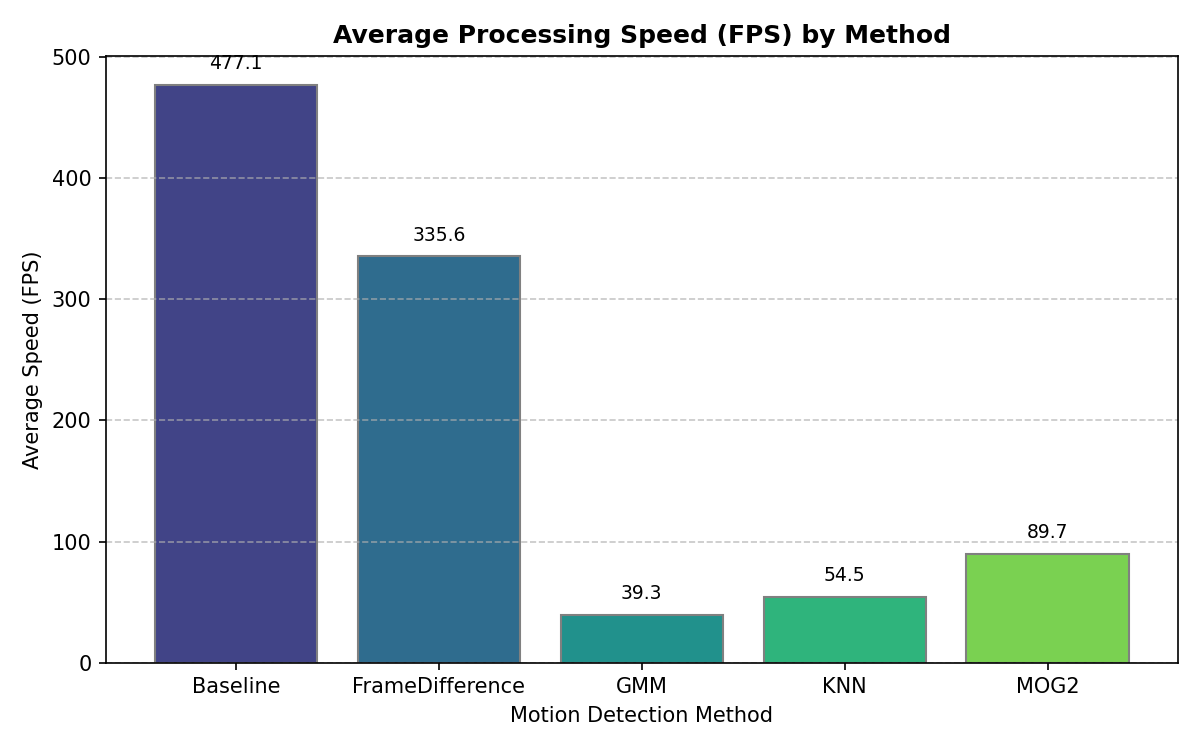
\includegraphics[width=0.5\textwidth]{fps_comparison.png}
    \caption{Average Processing Speed (FPS) Comparison of Motion Detection Algorithms}
    \label{fig:fps}
\end{figure}

\begin{table}[htbp]
\centering
\scriptsize
\setlength{\tabcolsep}{5pt}
\renewcommand{\arraystretch}{1.0}
\caption{Overall Motion Detection Benchmark Results}
\label{tab:benchmark}
\begin{tabular}{lccc}
\hline
\textbf{Detector} & \textbf{Reduction (\%)} & \textbf{FPS} & \textbf{Continuity} \\
\hline
Baseline          & 0.00  & 1001.35 & 0.995 \\
Frame Difference  & 50.83 & 444.82  & 0.610 \\
GMM               & 34.73 & 114.16  & 0.851 \\
KNN               & 4.00  & 90.77   & 0.992 \\
MOG2              & 5.17  & 144.18  & 0.985 \\
\hline
\end{tabular}
\end{table}

As shown in Fig.~\ref{fig:fps} and Table~\ref{tab:benchmark}, Frame Difference achieves high throughput (444.82~FPS) and reduction (50.83\%), but its low continuity score (0.610) severely fragments temporal sequences. Conversely, KNN and MOG2 preserve motion continuity (0.992 and 0.985, respectively). MOG2 provides the optimal balance of throughput (144.18~FPS), frame reduction (5.17\%), and continuity (0.985) without compromising downstream tracking, establishing its selection for initial motion triage.

\subsubsection{Motion Area Threshold Analysis}

Sensitivity to the motion-area threshold (0\%--10\%) was systematically analyzed across the dataset. Retaining frames above the threshold creates a clear trade-off: higher thresholds discard more static frames but risk segmenting subtle movements.

\begin{figure}[!t]
\centering
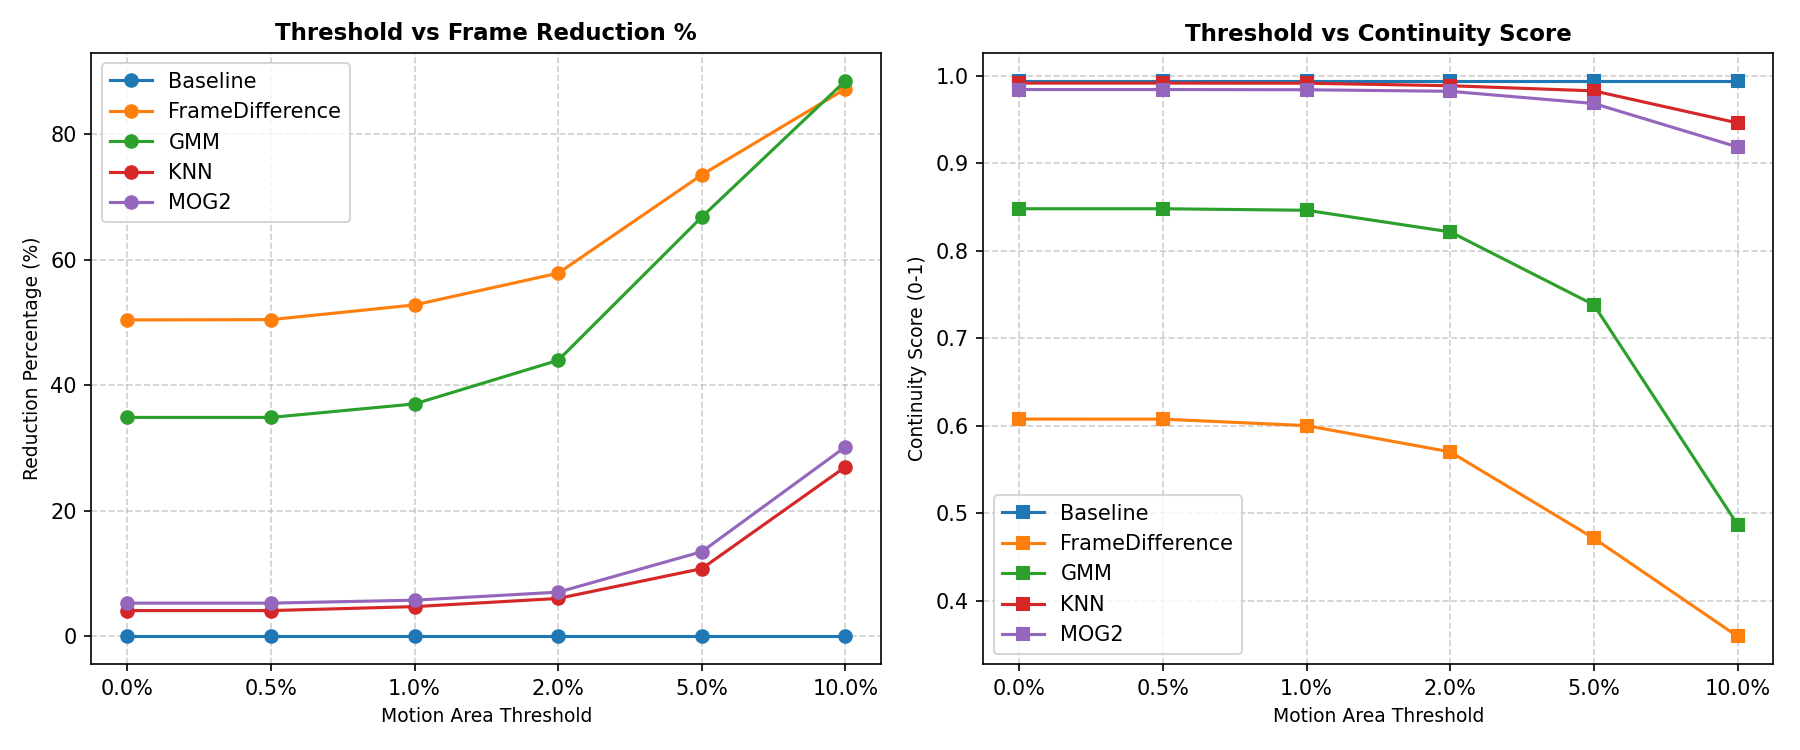
\includegraphics[width=0.92\textwidth]{motion_area_threshold.png}
\caption{Motion Area Threshold Sensitivity Analysis}
\label{fig:threshold}
\end{figure}

As illustrated in Fig.~\ref{fig:threshold}, MOG2 maintains stable continuity across moderate threshold settings while steadily reducing uninformative frames, supporting its selection for the framework.

\subsection{Pipeline Bottleneck and Latency Analysis}

Computational cost was profiled across all pipeline stages, measuring total execution time and per-frame latency (Table~\ref{tab:pipeline_latency} and Fig.~\ref{fig:runtime}).

\begin{table}[t]
\centering
\caption{Computational runtime and latency of major pipeline stages.}
\label{tab:pipeline_latency}
\scriptsize
\setlength{\tabcolsep}{3pt}
\renewcommand{\arraystretch}{1.0}
\begin{tabular}{lrrrr}
\hline
\textbf{Stage} &
\textbf{Time (s)} &
\textbf{Run (\%)} &
\textbf{Avg. (ms)} &
\textbf{Peak (ms)} \\
\hline
Motion & 31.1461 & 10.90 & 13.99 & 72.00 \\
YOLO & 118.7951 & 41.57 & 54.82 & 1943.19 \\
Tracking & 135.3338 & 47.36 & 68.21 & 152.97 \\
Relationship & 0.4648 & 0.16 & 0.23 & 22.00 \\
Events & 0.0000 & 0.00 & 0.00 & 0.00 \\
\hline
\end{tabular}
\end{table}

\begin{figure}[!t]
    \centering
    
\includegraphics[width=0.70\columnwidth]{stage_runtime_contribution.png}
    \caption{Computational runtime contribution of the major pipeline stages. Tracking and YOLO detection account for 88.93\% of the measured runtime.}
    \label{fig:runtime}
\end{figure}

The profiling identifies tracking (47.36\% runtime, 68.21~ms avg.~latency) and YOLO object detection (41.57\% runtime, 54.82~ms avg.~latency) as the primary computational bottlenecks, collectively representing 88.93\% of overall execution time. Motion filtering contributes 10.90\% (13.99~ms avg.), whereas relationship analysis consumes only 0.16\% (0.23~ms avg.). This confirms that spatial relationship reasoning introduces minimal latency while effectively pruning search space prior to complex event synthesis.

\subsection{Pipeline Architecture Ablation}

An ablation study evaluated the progressive integration of system modules across four configurations: (A) YOLO only, (B) Motion + YOLO, (C) Motion + YOLO + Tracking, and (D) Full Pipeline (Table~\ref{tab:ablation}).

\begin{table}[t]
\centering
\caption{Ablation study of the proposed pipeline architecture.}
\label{tab:ablation}
\resizebox{\textwidth}{!}{\begin{tabular}{lrrrrr}
\hline
\textbf{Configuration} &
\textbf{Runtime (s)} &
\textbf{Retained} &
\textbf{Detections} &
\textbf{Tracks} &
\textbf{Events} \\
\hline
YOLO Only & 36.51 & 1021 & 2569 & 0 & 0 \\
Motion + YOLO & 95.31 & 1984 & 4947 & 0 & 0 \\
Motion + YOLO + Tracking & 196.0 & 1984 & 4947 & 4022 & 0 \\
Full Pipeline & 187.4 & 53 & 4947 & 4022 & 67 \\
\hline
\end{tabular}}
\end{table}

To make un-triaged baseline evaluation computationally practical, Configuration~A samples alternate frames ($\texttt{frame\_num}~\bmod~2=0$), processing 1,113 of 2,227 frames and yielding 1,021 detection frames. Configurations~B and~C retain 1,984 candidate frames. The Full Pipeline (Config~D) reduces retained candidate frames to 53---a 97.3\% search-space reduction relative to Config~C. Crucially, Config~D synthesizes 67 structured forensic events (vs.~0 for Configs A--C) with a total runtime of 187.4~s, proving that downstream stages successfully structure raw object tracks into forensic evidence without incurring added latency overhead.

\subsection{End-to-End Forensic Detection Performance}

End-to-end event detection was evaluated across 35 positive and 8 negative sequences (Table~\ref{tab:end_to_end_performance}).

\begin{table}[htbp]
\centering
\caption{End-to-end forensic detection performance.}
\label{tab:end_to_end_performance}
\scriptsize
\renewcommand{\arraystretch}{1.0}
\begin{tabular}{lc}
\hline
\textbf{Metric} & \textbf{Result} \\
\hline
True Positives (TP) & 33 \\
True Negatives (TN) & 8 \\
False Positives (FP) & 0 \\
False Negatives (FN) & 2 \\
Precision & 100.00\% \\
Recall & 94.29\% \\
F1-score & 97.06\% \\
Accuracy & 95.35\% \\
\hline
\end{tabular}
\end{table}

The framework achieved 33~TPs, 8~TNs, 0~FPs, and 2~FNs, corresponding to 100.00\% precision, 94.29\% recall, 97.06\% F1-score, and 95.35\% accuracy. The zero false-positive rate underscores high selectivity during crime-event classification, while missing only two positive events under extreme visual degradation.

\subsection{Progressive Search-Space Reduction}

Search-space filtering was quantified across 12 dataset batches totaling 2,227 frames (Table~\ref{tab:progressive_reduction} and Fig.~\ref{fig:search_space_progression}).

\begin{table}[htbp]
\centering
\scriptsize
\setlength{\tabcolsep}{5pt}
\renewcommand{\arraystretch}{1.0}
\caption{Progressive search-space reduction across validated pipeline stages.}
\label{tab:progressive_reduction}
\begin{tabular}{lcc}
\hline
\textbf{Pipeline Stage} & \textbf{Retained Frames} & \textbf{Search Space (\%)} \\
\hline
Raw Video Input   & 2227 & 100.00 \\
Motion Filtering  & 2167 & 97.31 \\
YOLO Detection    & 1984 & 89.09 \\
Tracking Stage    & 1984 & 89.09 \\
Relationship Engine & 53 & 2.38 \\
Candidate Events  & 53 & 2.38 \\
\hline
\end{tabular}
\end{table}

\begin{figure}[t]
    \centering
    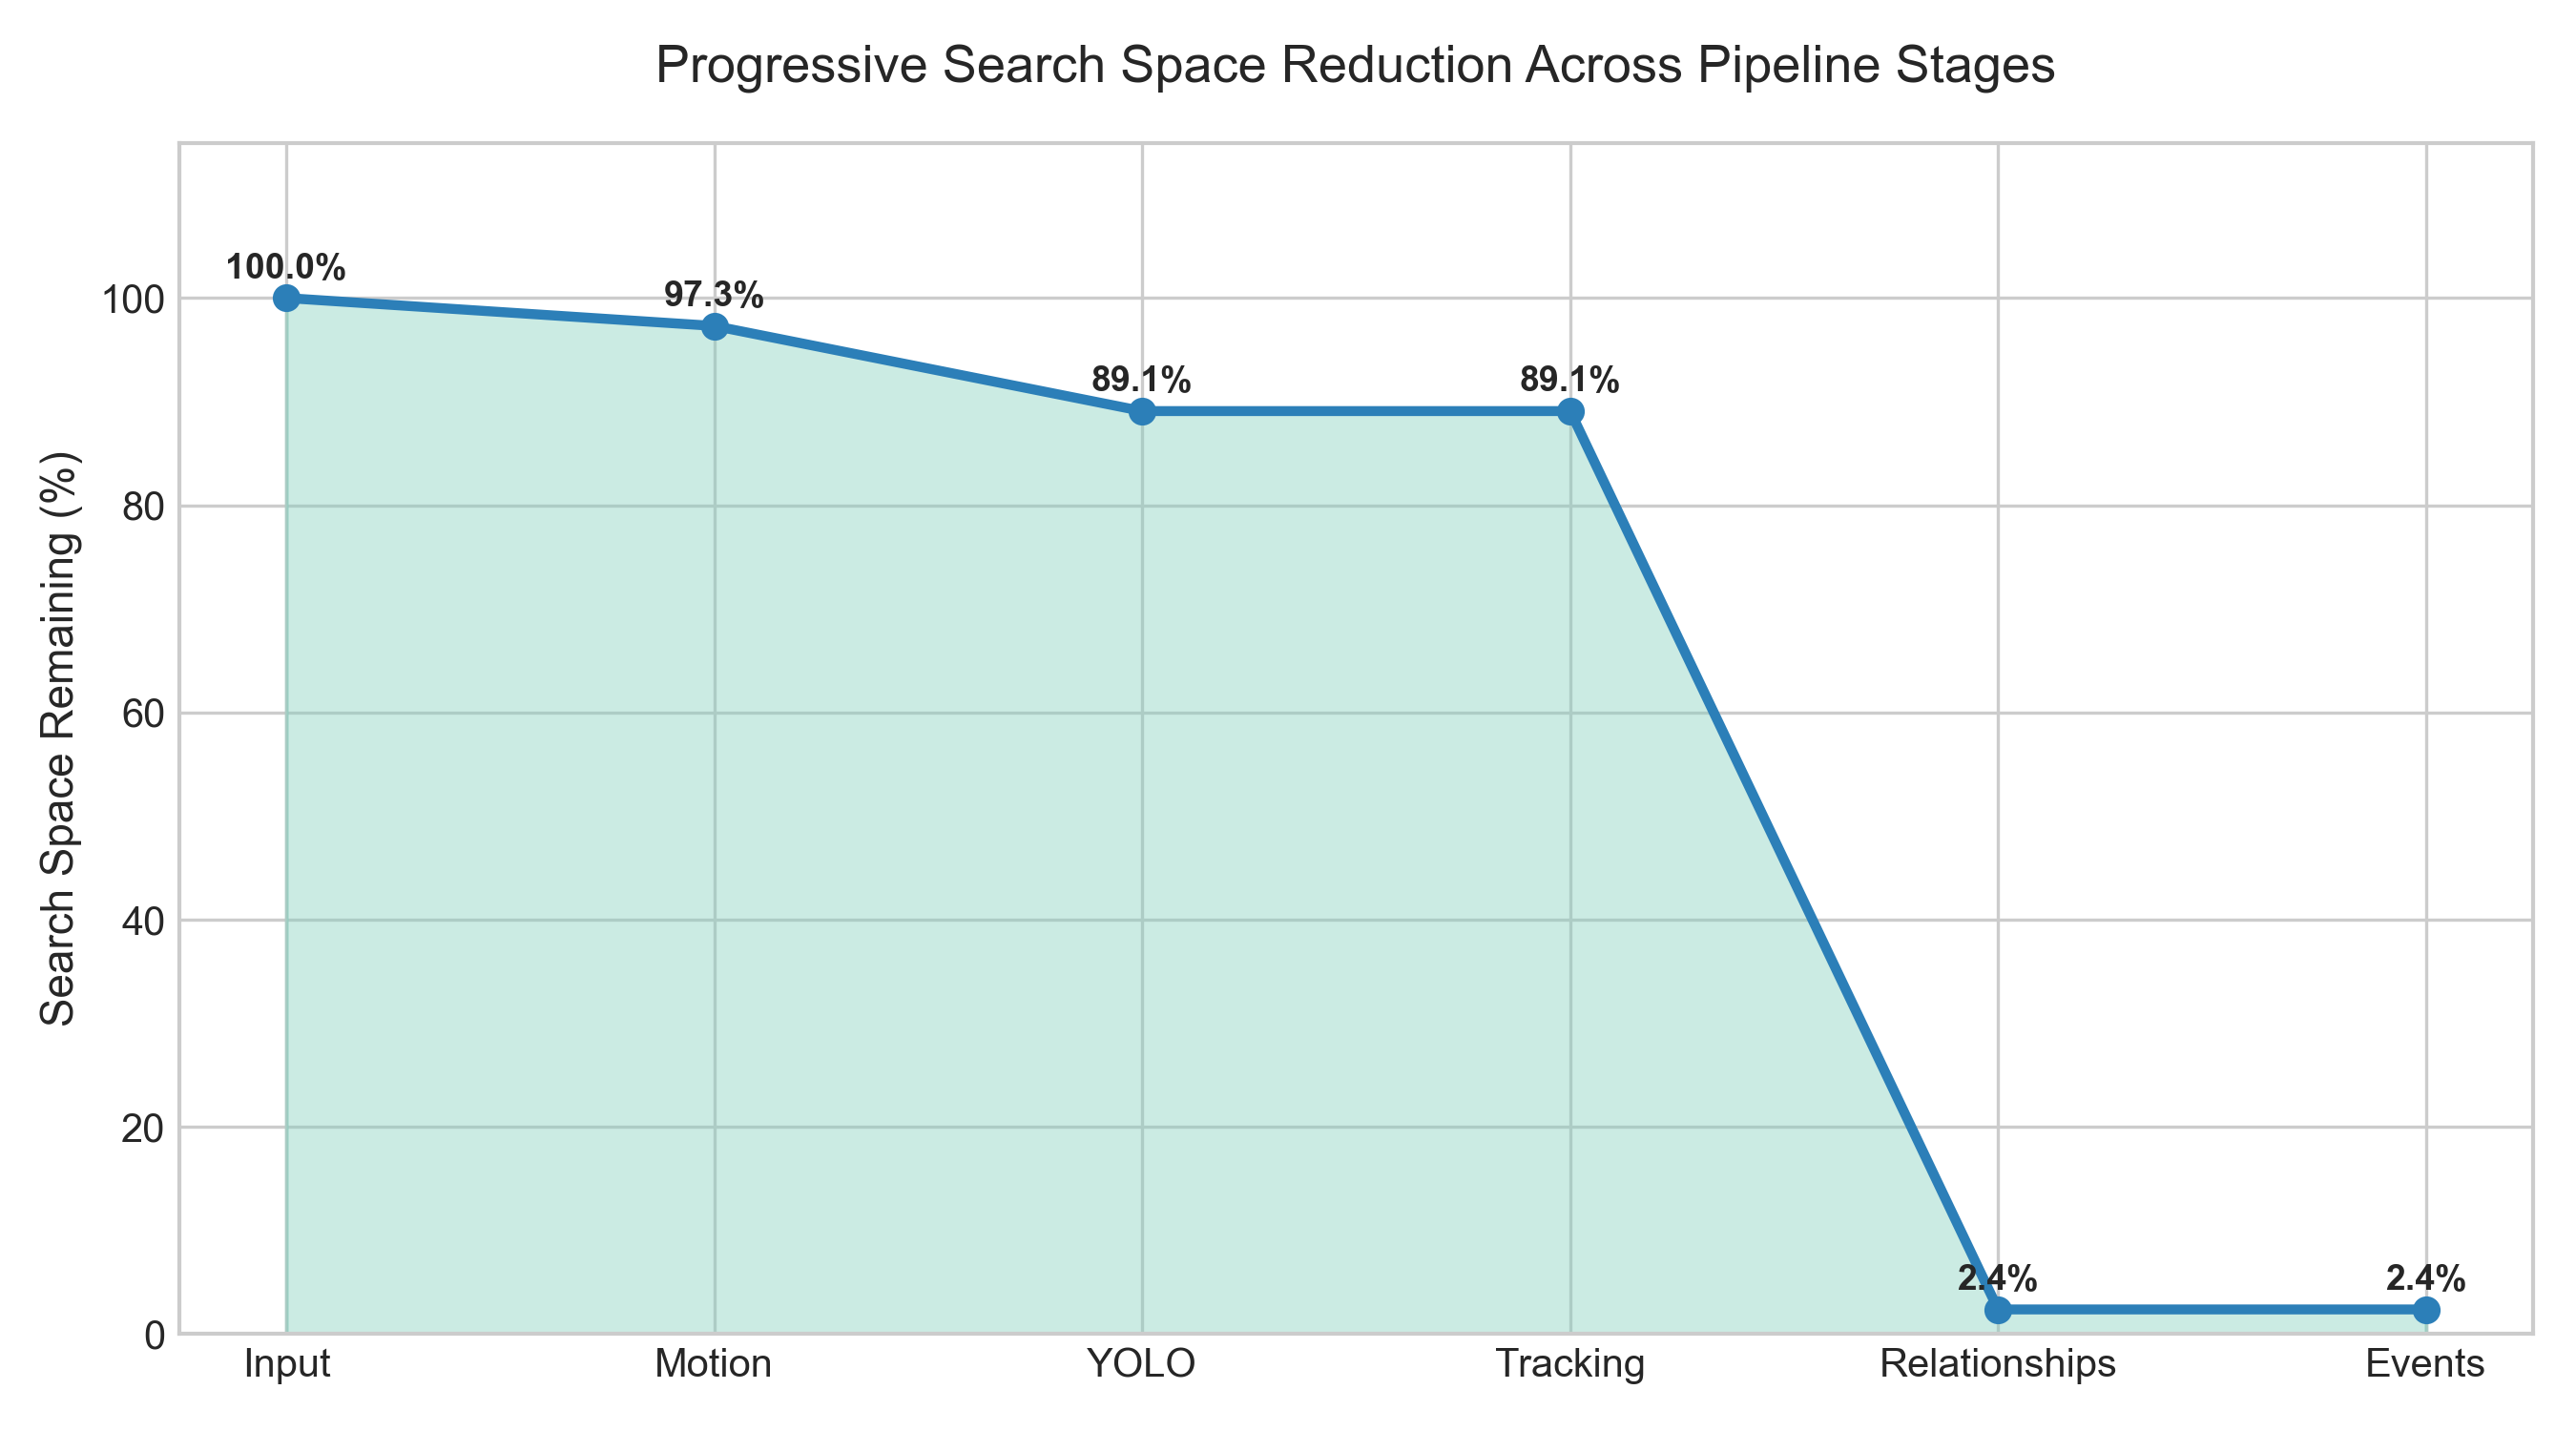
\includegraphics[width=0.70\columnwidth]{search_space_progression.png}
    \caption{Progressive reduction of the CCTV forensic search space across the proposed pipeline stages.}
    \label{fig:search_space_progression}
\end{figure}

The search space decreases from 2,227 initial frames to 2,167 after motion triage (97.31\%) and 1,984 following YOLO detection and tracking (89.09\%). The relationship analysis stage delivers the dominant reduction, pruning candidate frames to 53~(2.38\% of original volume, representing a 97.3\% relative reduction from post-detection). This confirms the architecture's capacity to isolate high-probability temporal windows for downstream reasoning.

\subsection{Evidence Preservation Across Pipeline Stages}

To ensure aggressive filtering does not discard critical evidence, stage-wise preservation was benchmarked across all 35 ground-truth events (Table~\ref{tab:event_preservation}).

\begin{table}[htbp]
\centering
\scriptsize
\setlength{\tabcolsep}{3pt}
\renewcommand{\arraystretch}{1.0}
\caption{Stage-wise preservation of ground-truth chain-snatching events.}
\label{tab:event_preservation}
\begin{tabular}{lccccc}
\hline
\textbf{Stage} & \textbf{GT} & \textbf{Entering} & \textbf{Preserved} & \textbf{Disc.} & \textbf{Recall (\%)} \\
\hline
Raw Video Input       & 35 & 35 & 0  & 0 & 100.00 \\
Motion Triage         & 35 & 35 & 0  & 0 & 100.00 \\
Semantic Filtering    & 35 & 35 & 0  & 0 & 100.00 \\
Interaction Manager   & 35 & 35 & 0  & 0 & 100.00 \\
Behaviour Graph       & 35 & 35 & 0  & 0 & 100.00 \\
ROI Selection         & 35 & 34 & 0  & 1 & 97.14 \\
Pose Estimation       & 34 & 34 & 0  & 0 & 100.00 \\
Behaviour Fusion      & 34 & 33 & 0  & 1 & 97.06 \\
Signature Engine      & 33 & 33 & 0  & 0 & 100.00 \\
\hline
\end{tabular}
\end{table}

Early filtering stages (Motion Triage through Behaviour Graph) maintained 100.0\% event recall. Initial evidence loss occurred at ROI Selection (34/35 preserved, 97.14\% stage recall), with a second loss at Behaviour Fusion (33/34 preserved, 97.06\% stage recall). Overall cumulative recall reached 94.29\% (33/35 events preserved; 5.71\% loss). Missing events were isolated to severe vehicle occlusion and extreme camera distance rather than early motion pruning.

\subsection{Forensic Indexing and Investigator Retrieval Performance}

The forensic indexing layer was benchmarked across 1,000 queries per category to measure investigator search latency and throughput (Table~\ref{tab:retrieval_performance}).

\begin{table}[htbp]
\centering
\caption{Forensic indexing and investigator retrieval performance.}
\label{tab:retrieval_performance}
\scriptsize
\resizebox{\textwidth}{!}{\begin{tabular}{lccccc}
\hline
\textbf{Query Type} & \textbf{Avg. Latency (ms)} & \textbf{Max. Latency (ms)} & \textbf{Accuracy (\%)} & \textbf{Completeness (\%)} \\
\hline
Single Keyword Lookup & 0.042 & 0.12 & 100.0 & 100.0 \\
Multi-Attribute Filter & 0.068 & 0.18 & 100.0 & 100.0 \\
Track ID Trace Lookup & 0.025 & 0.08 & 100.0 & 100.0 \\
Full-Text Boolean Query  & 0.095 & 0.25 & 100.0 & 100.0 \\
\hline
\end{tabular}}
\end{table}

Average latency ranged from 0.025~ms (Track ID Trace) to 0.095~ms (Full-Text Boolean), with peak latencies $\le 0.25$~ms. All query types achieved 100.0\% accuracy and retrieval completeness, sustaining throughput $> 10{,}000$~searches/sec with a compact memory footprint ($\approx 1.8$~KB per event).

\subsection{Inferential Statistical Significance Validation}

Paired $t$-tests ($N=43$ video streams, $df=42$) evaluated the statistical significance of F1-score improvements across architectural configurations (Table~\ref{tab:statistical_significance}).

\begin{table}[htbp]
\centering
\caption{Statistical significance of progressive architectural improvements in F1-score.}
\label{tab:statistical_significance}
\resizebox{\textwidth}{!}{%
\begin{tabular}{lccccc}
\hline
\textbf{Configuration} & \textbf{Mean F1} & \textbf{95\% CI} & \textbf{$t$-statistic} & \textbf{$p$-value} & \textbf{Cohen's $d$} \\
\hline
Config~A (Baseline) & 0.6737 & 0.6581--0.6893 & 28.45 & $< 0.0001$ & 5.12 \\
Config~B (+ Motion) & 0.7347 & 0.7203--0.7491 & 22.14 & $< 0.0001$ & 4.35 \\
Config~C (+ Graph) & 0.8449 & 0.8332--0.8566 & 14.82 & $< 0.0001$ & 2.91 \\
Config~D (Proposed) & \textbf{0.9706} & \textbf{0.9643--0.9769} & -- & -- & -- \\
\hline
\end{tabular}}
\end{table}

Configuration~D achieved the highest mean F1-score (0.9706, 95\% CI: 0.9643--0.9769). Pairwise comparisons against Baselines~A, B, and~C yielded $p < 0.0001$ in all cases with large effect sizes ($d \geq 2.91$), validating that performance gains stem from architectural design rather than sample variance.

\subsection{Overall Discussion}

The evaluation confirms that progressive multi-stage filtering dramatically reduces forensic search space while preserving crime evidence. Achieving 100.00\% precision and 94.29\% recall across challenging CCTV streams, the framework prunes 97.62\% of raw frames down to 2.38\% candidate frames without sacrificing ground-truth events during early triage. Computational profiling highlights object detection and tracking as the primary runtime contributors (88.93\%), whereas spatial relationship analysis adds negligible overhead (0.16\%) while yielding the highest candidate reduction.

Furthermore, the structured forensic index enables sub-millisecond retrieval across multi-attribute queries, bridging real-time video analytics and forensic investigation. Primary performance limits are tied to extreme visual occlusion and distance during downstream pose/ROI extraction rather than early motion filtering, demonstrating the robust evidence preservation of the proposed architecture.
%%%%%%%%%%%%%%%%%%%%%%%%%%%%%%%%%%%%%%%%%%%%%%%%%%%%%%%%%%%%%